%%%%%%%%%%%%%%%%%%%%%%%%%%%%%%%%%%%%%%%%%
% Beamer Presentation
% LaTeX Template
% Version 1.0 (10/11/12)
%
% This template has been downloaded from:
% http://www.LaTeXTemplates.com
%
% License:
% CC BY-NC-SA 3.0 (http://creativecommons.org/licenses/by-nc-sa/3.0/)
%
%%%%%%%%%%%%%%%%%%%%%%%%%%%%%%%%%%%%%%%%%

%----------------------------------------------------------------------------------------
%	PACKAGES AND THEMES
%----------------------------------------------------------------------------------------

\documentclass{beamer}

\mode<presentation> {

% The Beamer class comes with a number of default slide themes
% which change the colors and layouts of slides. Below this is a list
% of all the themes, uncomment each in turn to see what they look like.

\usetheme{default}
%\usetheme{AnnArbor}
%\usetheme{Antibes}
%\usetheme{Bergen}
%\usetheme{Berkeley}
%\usetheme{Berlin}
%\usetheme{Boadilla}
%\usetheme{CambridgeUS}
%\usetheme{Copenhagen}
%\usetheme{Darmstadt}
%\usetheme{Dresden}
%\usetheme{Frankfurt}
%\usetheme{Goettingen}
%\usetheme{Hannover}
%\usetheme{Ilmenau}
%\usetheme{JuanLesPins}
%\usetheme{Luebeck}
%\setheme{Madrid}
%\usetheme{Malmoe}
%\usetheme{Marburg}
%\usetheme{Montpellier}
%\usetheme{PaloAlto}
%\usetheme{Pittsburgh}
%\usetheme{Rochester}
%\usetheme{Singapore}
%\usetheme{Szeged}
%\usetheme{Warsaw}

% As well as themes, the Beamer class has a number of color themes
% for any slide theme. Uncomment each of these in turn to see how it
% changes the colors of your current slide theme.

%\usecolortheme{albatross}
%\usecolortheme{beaver}
%\usecolortheme{beetle}
%\usecolortheme{crane}
%\usecolortheme{dolphin}
%\usecolortheme{dove}
%\usecolortheme{fly}
%\usecolortheme{lily}
%\usecolortheme{orchid}
%\usecolortheme{rose}
%\usecolortheme{seagull}
\usecolortheme{seahorse}
%\usecolortheme{whale}
%\usecolortheme{wolverine}

%\setbeamertemplate{footline} % To remove the footer line in all slides uncomment this line
\setbeamertemplate{footline}[frame number] % To replace the footer line in all slides with a simple slide count uncomment this line

%\setbeamertemplate{navigation symbols}{} % To remove the navigation symbols from the bottom of all slides uncomment this line
}

\usepackage{graphicx} % Allows including images
\usepackage{booktabs} % Allows the use of \toprule, \midrule and \bottomrule in tables
\usepackage{tikz}
\usetikzlibrary{matrix}
\usepackage{listings}
\usepackage{xcolor}
\usepackage{IEEEtrantools}
\usepackage{amsmath}
\usepackage{amssymb}
\usepackage{dsfont}
\usepackage{longtable}
\usepackage{mathtools}
\usepackage{iris}
\usepackage{arydshln}
\usepackage[thinlines]{easytable}

\newcommand{\sep}{-\kern-.6em\raisebox{-.659ex}{*}\ }
\newcommand{\bupd}[1]{=\kern-.6em\{#1\}\ \kern-.9em =\ \kern-.8em\raisebox{-.659ex}{*}\ }
\newcommand{\fupd}{=\kern-.3em=\ \kern-.8em\raisebox{-.659ex}{*}\ }
\newcommand{\nfupd}{=\kern-.6em \backslash\ \kern-.9em=\ \kern-.8em\raisebox{-.659ex}{*}\ }

\newcommand{\bigsep}{\mathop{\scalebox{2.5}{\raisebox{-0.4ex}{$*$}}}}%
\newcommand\myeq[1]{\stackrel{\mathclap{\normalfont\mbox{#1}}}{=}}


%\newcommand{\ra}[1] {
%  \begin{tikzpicture}
%        \node[draw,dashed] {#1};
%    \end{tikzpicture}}
    
\newcommand{\inv}[1] {
  \begin{tikzpicture}
        \node[draw] {#1};
    \end{tikzpicture}}
    
\newcommand{\interp}[2]{(#1)(#2)}
\newcommand\sepimp{\mathrel{-\mkern-6mu*}}

\usetikzlibrary{decorations.pathreplacing}

\newcommand\MemoryLayout[1]{
  \begin{tikzpicture}[scale=0.3]
     \draw[thick](0,0)--++(0,1);
     \foreach \pt/\col/\lab [remember=\pt as \tp (initially 0)] in {#1} {
     \if\lab\relax\relax\else
         \draw[thick,decorate, decoration={brace,amplitude=4mm}]
            (-\tp,-0.2)--node[below=4mm]{\lab} (-\pt+2,-0.2);
            \draw[fill=\col] (-\tp,0) rectangle (-\pt+2,1);
       \fi
       \foreach \a in {\tp,...,\pt} {
          \draw(-\a,0) rectangle ++(-1,1);
       }
       \draw[thick](-\pt,0)--++(0,1);
       
     }
     \node at (-4.5,0.6) {\small B};
  \end{tikzpicture}
}

\def\world{\emph{World}}
\def\word{\emph{Word}}

 
\definecolor{codegreen}{rgb}{0,0.6,0}
\definecolor{codegray}{rgb}{0.5,0.5,0.5}
\definecolor{codepurple}{rgb}{0.58,0,0.82}
\definecolor{backcolour}{rgb}{0.95,0.95,0.92}
 
\lstdefinestyle{mystyle}{
    backgroundcolor=\color{backcolour},   
    commentstyle=\color{codegreen},
    keywordstyle=\color{magenta},
    numberstyle=\tiny\color{codegray},
    stringstyle=\color{codepurple},
    basicstyle=\ttfamily\footnotesize,
    breakatwhitespace=false,         
    breaklines=true,                 
    captionpos=b,                    
    keepspaces=true,                 
    numbers=left,                    
    numbersep=5pt,                  
    showspaces=false,                
    showstringspaces=false,
    showtabs=false,                  
    tabsize=2
}
 
\lstset{style=mystyle,xleftmargin=.2\textwidth, xrightmargin=.2\textwidth}

\setbeamercovered{transparent}
\setbeamercolor{alerted text}{fg=red}

\AtBeginSection[]{
  \begin{frame}
  \vfill
  \centering
  \begin{beamercolorbox}[sep=8pt,center,shadow=true,rounded=true]{title}
    \usebeamerfont{title}\insertsectionhead\par%
  \end{beamercolorbox}
  \vfill
  \end{frame}
}

\AtBeginSubsection[]
{
    \begin{frame}
  	\vfill
  	\centering
  	\begin{beamercolorbox}[sep=8pt,center,shadow=true,rounded=true]{title}
    \usebeamerfont{title}\insertsubsectionhead\par%
  	\end{beamercolorbox}
  	\vfill
  \end{frame}
}
%----------------------------------------------------------------------------------------
%	TITLE PAGE
%----------------------------------------------------------------------------------------

\title[Capability Machine in Iris]{Implementing a Capability Machine model into Iris} % The short title appears at the bottom of every slide, the full title is only on the title page

\author{\textbf{A\"{i}na Linn Georges} \hspace{1cm} Alix Trieu \hspace{1cm} Lars Birkedal} % Your name
\institute[Aarhus University] % Your institution as it will appear on the bottom of every slide, may be shorthand to save space
{
Aarhus University \\ % Your institution for the title page
\medskip
\textit{ageorges@cs.au.dk} % Your email address
}
\date{\today} % Date, can be changed to a custom date

\begin{document}

\begin{frame}
\titlepage % Print the title page as the first slide
\end{frame}

\begin{frame}
\frametitle{Introduction}

\begin{itemize}
	\item<1> Capability machines allow for fine grained control over pointer permissions 
	\item<2> Good target for secure compilation
	\item<3> In particular: we are interested in enforcing certain higher level abstractions such as \textit{local state encapsulation} as \textit{well-bracketed control flow} at the lowest level of the machine
	\item<4> We need tools to reason about these subtle properties in a language that does not enforce them
	\item<5> These tools are elaborate and complex: we want to mechanize them, and facilitate the process of using them
\end{itemize}

\textit{Reasoning about a Machine with Local Capabilities}: \cite{p1}

\end{frame}

%----------------------------------------------------------------------------------------
%	PRESENTATION SLIDES
%----------------------------------------------------------------------------------------

%\begin{frame}
%\frametitle{Overview} % Table of contents slide, comment this block out to remove it
%\tableofcontents[hideallsubsections]
% % Throughout your presentation, if you choose to use \section{} and \subsection{} commands, these will automatically be printed on this slide as an overview of your presentation
%\end{frame}

%------------------------------------------------
\section{Capability Machines} % Sections can be created in order to organize your presentation into discrete blocks, all sections and subsections are automatically printed in the table of contents as an overview of the talk
%------------------------------------------------


\begin{frame}
\frametitle{Capability Machine}

\uncover<5->{\textbf{Capability: } An unforgeable token of authority
\\[1cm]}
\begin{columns}[c]

\column{.45\textwidth} % Left column and width
\begin{tikzpicture}
    \node<1> (img1) {
\includegraphics[scale=0.7]{images/cap_1.pdf}};
    \node<2> (img2) {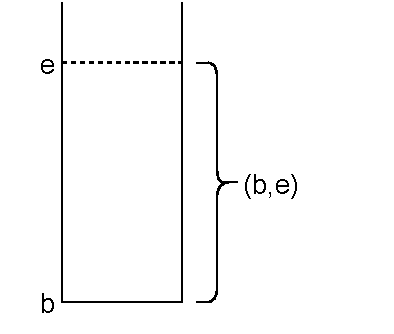
\includegraphics[scale=0.7]{images/cap_2.pdf}};
    \node<3> (img3) {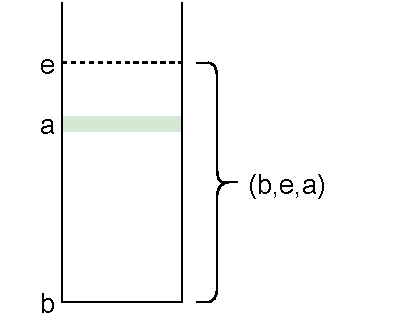
\includegraphics[scale=0.7]{images/cap_3.pdf}};
    \node<4-> (img4) {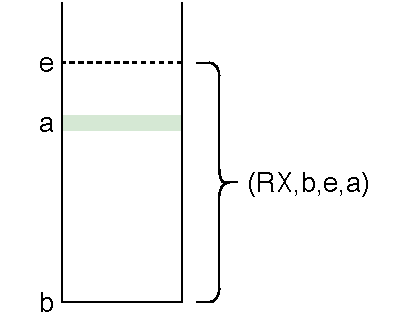
\includegraphics[scale=0.7]{images/cap_4'.pdf}};
\end{tikzpicture}

\column{.5\textwidth} % Right column and width
\uncover<4->{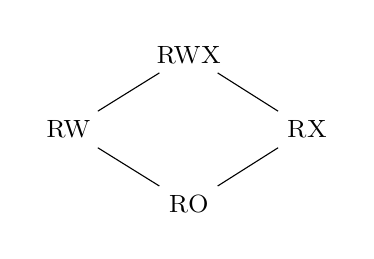
\begin{tikzpicture}

\matrix (a) [matrix of math nodes, ampersand replacement=\&, column sep=0.6cm, row sep=0.5cm]{
\& \textsc{\small RWX} \&\\
\textsc{\small RW}  \& \& \textsc{\small RX}  \\
\& \textsc{\small RO} \&\\};

\foreach \i/\j in {1-2/2-1, 1-2/2-3, 2-1/3-2, 2-3/3-2}
    \draw (a-\i) -- (a-\j);
%
\end{tikzpicture}}

\end{columns}
\only<2-4>{
\begin{itemize}
	\item \only<2>{Range}
			  \only<3>{Address}
			  \only<4>{Permission}
\end{itemize}}

\end{frame}

%------------------------------------------------
%\subsection{Enforcing Local State Encapsulation using Capabilities} % A subsection can be created just before a set of slides with a common theme to further break down your presentation into chunks
%
%\begin{frame}[fragile]
%\frametitle{Capability Safety}
%\textbf{Local State Encapsulation}
%\\[1cm]
%\begin{columns}[c]
%
%\column{.45\textwidth} % Left column and width
%\begin{tikzpicture}
%    \node<1> (img1) {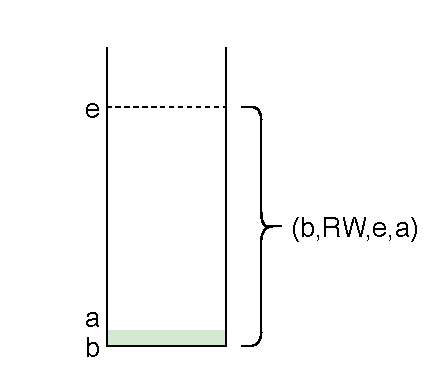
\includegraphics[scale=0.7]{images/wbcf_1.pdf}};
%    \node<2> (img2) {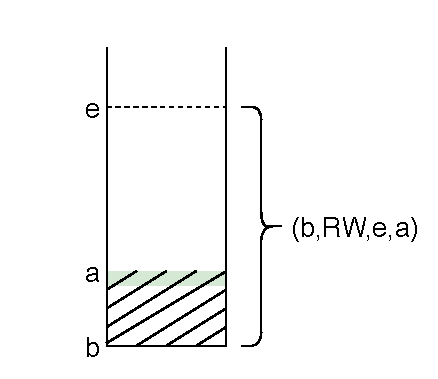
\includegraphics[scale=0.7]{images/wbcf_2.pdf}};
%    \node<3> (img3) {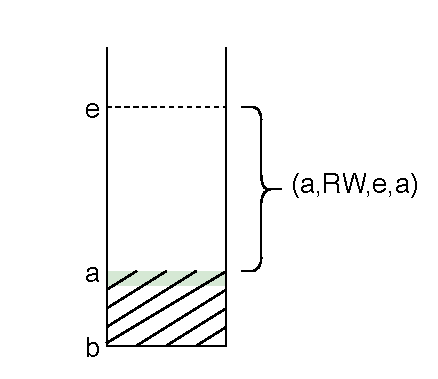
\includegraphics[scale=0.7]{images/wbcf_3.pdf}};
%\end{tikzpicture}
%
%\column{.5\textwidth} % Right column and width
%\begin{center}
%\begin{lstlisting}
%push r_stk 1
%scall r 
%pop r_stk r_1
%assert r_1 1
%halt
%\end{lstlisting}
%\end{center}
%
%
%\end{columns}
%\end{frame}

%------------------------------------------------
\subsection{Enforcing Well-Bracketed Control Flow using Capabilities} % A subsection can be created just before a set of slides with a common theme to further break down your presentation into chunks

\begin{frame}[fragile]
\frametitle{Capability Safety}
\textbf{Well-Bracketed Control Flow}
\\[1cm]
\begin{columns}[c]

\column{.45\textwidth} % Left column and width
\begin{tikzpicture}
    \node<1> (img1) {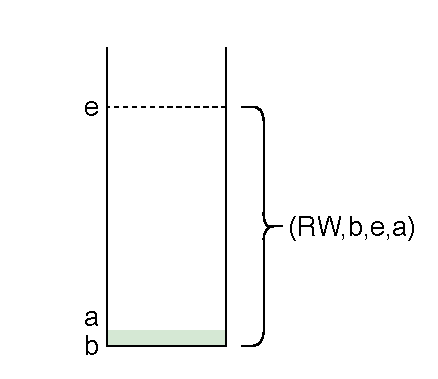
\includegraphics[scale=0.7]{images/wbcf_1'.pdf}};
    \node<2> (img2) {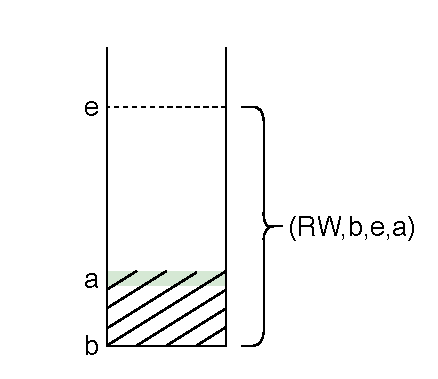
\includegraphics[scale=0.7]{images/wbcf_2'.pdf}};
    \node<3> (img3) {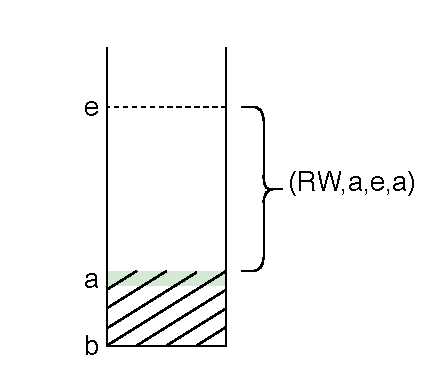
\includegraphics[scale=0.7]{images/wbcf_3'.pdf}};
    \node<4> (img4) {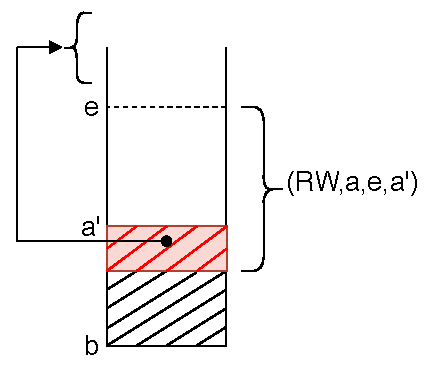
\includegraphics[scale=0.7]{images/wbcf_4'.pdf}};
    \node<5> (img5) {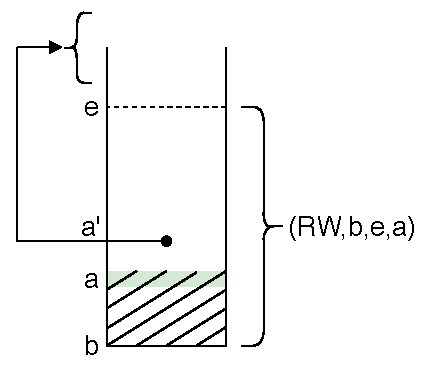
\includegraphics[scale=0.7]{images/wbcf_5'.pdf}};
    \node<6> (img6) {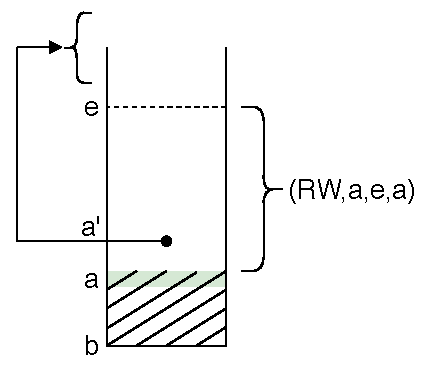
\includegraphics[scale=0.7]{images/wbcf_6'.pdf}};
\end{tikzpicture}

\column{.5\textwidth} % Right column and width
\begin{center}
\begin{lstlisting}
push r_stk 1
scall r
pop r_stk r_1
assert r_1 1
push r_stk 2
scall r 
halt
\end{lstlisting}
\end{center}

\end{columns}

\begin{itemize}
	\item \only<1>{We start with a stack with range b to e}
			  \only<2>{Push some local state}
			  \only<3>{Prepare adversary stack}
			  \only<4>{Adversary possesses a return capability}
			  \only<5>{Once jumped to we get back original stack - we pop the stack and assert that local state did not change}
			  \only<6>{Prepare the adversary stack for second call}
\end{itemize}
\end{frame}

%------------------------------------------------
\subsection{Local Capabilities}
\begin{frame}
\frametitle{Local Capabilities}

\begin{center} (p,\textbf{Local},b,e,a) \hspace{2cm} (p,\textbf{Global},b,e,a) \end{center}

\uncover<2->{

\begin{tikzpicture}

\matrix (a) [matrix of math nodes, ampersand replacement=\&, column sep=0.6cm, row sep=0.5cm]{
\& \& \textsc{\small RWLX} \& \& \& \\
\& \textsc{\small RWX} \& \& \textsc{\small RWL} \& \& \\
\textsc{\small RX} \& \& \textsc{\small RW}  \&  \\
\& \textsc{\small RO} \& \\};

\foreach \i/\j in {1-3/2-2, 1-3/2-4, 2-2/3-1, 2-4/3-3, 2-2/3-3, 3-1/4-2, 3-3/4-2}
    \draw (a-\i) -- (a-\j);
%
\end{tikzpicture}
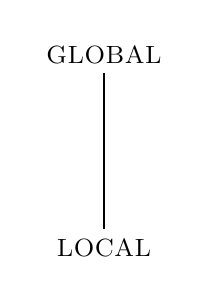
\begin{tikzpicture}

\matrix (a) [matrix of math nodes, ampersand replacement=\&, column sep=0.6cm, row sep=0.5cm]{
\textsc{\small GLOBAL}\\ \\ \\ \\
\textsc{\small LOCAL}\\};

\foreach \i/\j in {1-1/5-1}
    \draw (a-\i) -- (a-\j);
%
\end{tikzpicture}
\begin{itemize}
	\item Local capabilities can only be stored where you have write local permission
\end{itemize}
}

\end{frame}

\begin{frame}
\frametitle{Calling Convention}
\begin{tikzpicture}
    \node<1> (img1) {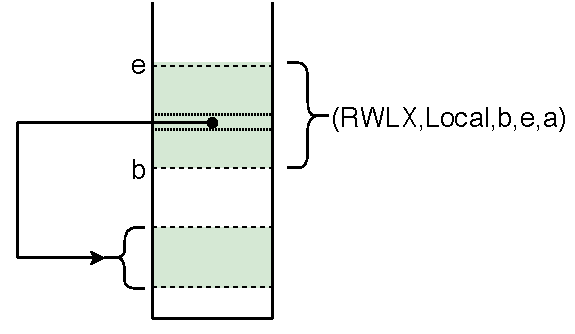
\includegraphics[scale=0.7]{images/calling_1.pdf}};
    \node<2> (img2) {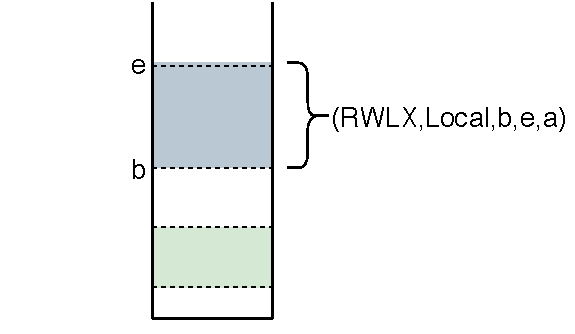
\includegraphics[scale=0.7]{images/calling_2.pdf}};
\end{tikzpicture}
%
%\begin{longtable}[c]{|l|l|}
%\hline
%\texttt{r\_stk} & $(RWLX,Local,b,e,a)$ \\ \hline
%\endfirsthead
%%
%\endhead
%\end{longtable}
\begin{itemize}
	\item We want the adversary to lose any temporary capabilities (such as return capabilities) upon return of a function call
\end{itemize}
\end{frame}

%------------------------------------------------
\section{Reasoning about Capability Safety}

\begin{frame}
\frametitle{Expressing Capability Safety}

\begin{itemize}
	\item<2-> using a program logic 
	\item<3-> using a logical relation to capture invariants on the type system
	\item<4-> \textbf{using a logical relation on an \emph{untyped} (or \emph{uni-typed}) language to capture semantic properties of the language}
\end{itemize}

\end{frame}

\begin{frame}
\frametitle{Step-indexed Kripke Logical Relation}
 
$$ \mathcal{V}\uncover<2->{(W)}\triangleq~\{\uncover<5->{{\color{red}n}}, (RW, g, b, e, a) | \only<1-2>{\cdots} \only<3->{\exists r, W(r) \only<3-4>{=} \only<5->{\myeq{\small {\color{red} n}}} \iota_{[b,e]}} \} \cup \cdots $$
 
 \begin{itemize}
 	\item<4-> World-circularity problem
 		\begin{itemize}
 			\item<5-> {\color{red} Step indexing}
 		\end{itemize}
 	\item<6-> The world may evolve: we need future world relation
 		\begin{itemize}
 			\item<7-> Local capabilities are revoked whereas Global capabilities are not, \textit{the relation needs to model this distinction}:
 			$$ \sqsupseteq_{pub} \hspace{1 cm} and \hspace{1 cm} \sqsupseteq_{priv} $$
 		\end{itemize}
 \end{itemize}

\end{frame}

\begin{frame}
\frametitle{Expressing Capability Safety in Iris - an Iris primer}

\textbf{Iris:} Higher-order Concurrent Separation Logic Framework
\begin{itemize}
	\item<2-> Foundational
	\item<3-> Implemented in Coq -- equipped with an interactive proof mode
	\item<4-> Framework -- embed any language and its operational semantics into Iris
	\item<5-> Comes equipped with: 
		\begin{itemize}
			\item<5-> Invariants
			\item<6-> Ghost state
			\item<7-> Always and Later Modalities
		\end{itemize}
\end{itemize}

\uncover<8->{We can take advantage of Iris' step-indexed model and invariants to mechanize step-indexed Kripke logical relations with recursive worlds in a succinct and elegant way.}

\end{frame}

\begin{frame}
\frametitle{Expressing Capability Safety in Iris - Challenges}

\begin{itemize}
	\item Region invariants: Iris invariants
	\item Future world relation: frame preserving updates and world satisfaction 
	\item Step indexing: later modality
\end{itemize}

\textbf{Challenges}
\begin{itemize}
	\item<2-> Iris was designed with more high level languages in mind, how do we embed a low level machine language into Iris
	\item<3-> Iris abstracts away certain details we want to reason about directly
	\item<4-> There is only one frame preserving update, we need to distinguish between two future world relations
\end{itemize}

\end{frame}

\begin{frame}
\frametitle{Expressing Capability Safety in Iris}

\textbf{Roadmap}
	\begin{itemize}
		\item<2> embed the language into Iris
		\item<3> define a program logic by proving hoare triples
		\item<4> define the logical relation -- using Iris tools to solve the world circularity problem
		\item<5> prove the fundamental theorem of logical relations
		\item<6> use the logical relation to prove examples that rely on local state encapsulation and well-bracketed control flow with calls to unknown adversary
	\end{itemize}

\end{frame}


%------------------------------------------------
\section{A Unary Logical Relation for Reasoning about Semantic Properties of an Untyped Language}
%------------------------------------------------

%------------------------------------------------
\subsection{The Value Relation}

\begin{frame}[fragile]
\frametitle{The Value Relation}
\begin{center}
\textbf{A unary logical relation of an un-typed language}
\end{center}

$$\mathcal{V} : \only<6->{{\color{red}STS} \rightarrow~} 
			Word \rightarrow iProp~\Sigma $$
\\[1em]
\uncover<3->{\textbf{Challenge: }distinguish between Local and Global capabilities:
\begin{itemize}
	\item<4-> At the level of the value relation
	\item<5-> Model revocation
\end{itemize}
}
\uncover<6->{{\color{red} STS}: A collection of state transition systems}

\uncover<2->{
$$  \mathcal{V}\only<6->{{\color{red} (\Sigma)}}((\text{\tiny{RW}},g),b,e,a) \triangleq~ \bigsep_{a \in [b,e]} \fbox{$\exists w, a \mapsto_a [RW] w * \mathcal{V}\only<5->{{\color{red} (\Sigma)}}(w)$}$$}


\end{frame}

\begin{frame}
\frametitle{From World to state transition system collection}
On paper: 
\begin{align*}
	\text{Region} =~&\{Revoked\}~\uplus \\
						     &\{Temporary\} \times {\color{red} \text{State} \times \text{Rels}} \\ 
						     &\times (\text{State} \rightarrow (Wor \xrightarrow[\sqsupseteq_{pub}]{mon, ne} \text{UPred(MemSeg)}))~\uplus \\
						     &\{Permanent\} \times {\color{red} \text{State} \times \text{Rels}}  \\ 
						     &\times (\text{State} \rightarrow (Wor \xrightarrow[\sqsupseteq_{priv}]{mon, ne} \text{UPred(MemSeg)})) \\
	\text{World} =~&\mathds{N} \rightharpoonup \text{Region}
\end{align*}
In the Iris mechanization, we use a collection of state transition systems: 
$$\Sigma: \mathds{N} \rightharpoonup States \times \mathds{N} \rightharpoonup Rels $$
\uncover<2->{The world circularity problem is now handled using Iris invariants and saved predicates.}
	
\end{frame}

\begin{frame}
\frametitle{Standard STS}

$$\Sigma: \mathds{N} \rightharpoonup States \times \mathds{N} \rightharpoonup Rels $$

\begin{center}
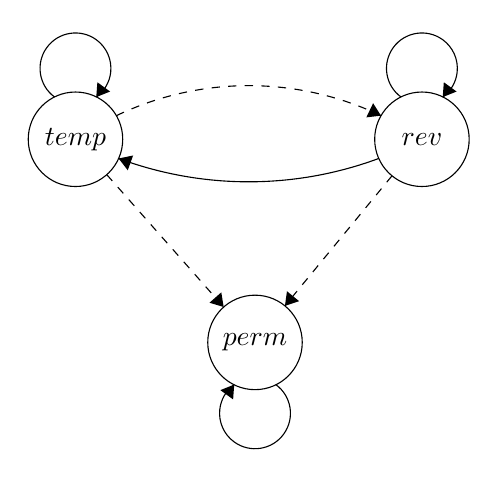
\begin{tikzpicture}[scale=0.2]
\tikzstyle{every node}+=[inner sep=0pt]
\draw [black] (17.8,-20.1) circle (3);
\draw (17.8,-20.1) node {$temp$};
\draw [black] (39.8,-20.1) circle (3);
\draw (39.8,-20.1) node {$rev$};
\draw [black] (29.2,-33) circle (3);
\draw (29.2,-33) node {$perm$};
\draw [black,dashed] (20.396,-18.602) arc (115.58004:64.41996:19.465);
\fill [black] (37.2,-18.6) -- (36.7,-17.81) -- (36.27,-18.71);
\draw [black] (37.061,-21.318) arc (-69.63899:-110.36101:23.742);
\fill [black] (20.54,-21.32) -- (21.12,-22.07) -- (21.46,-21.13);
\draw [black,dashed] (19.79,-22.35) -- (27.21,-30.75);
\fill [black] (27.21,-30.75) -- (27.06,-29.82) -- (26.31,-30.48);
\draw [black,dashed] (37.9,-22.42) -- (31.1,-30.68);
\fill [black] (31.1,-30.68) -- (32,-30.38) -- (31.23,-29.75);
\draw [black] (16.477,-17.42) arc (234:-54:2.25);
\fill [black] (19.12,-17.42) -- (20,-17.07) -- (19.19,-16.48);
\draw [black] (38.477,-17.42) arc (234:-54:2.25);
\fill [black] (41.12,-17.42) -- (42,-17.07) -- (41.19,-16.48);
\draw [black] (30.523,-35.68) arc (54:-234:2.25);
\fill [black] (27.88,-35.68) -- (27,-36.03) -- (27.81,-36.62);
\end{tikzpicture}
\end{center}

\begin{itemize}
	\item Dotted lines: private transitions
	\item Continuous lines: public transitions
\end{itemize}

\end{frame}

%------------------------------------------------
%\section{What's new/contributions}
%------------------------------------------------

\begin{frame}
\frametitle{What's new}

\textbf{What's new: capability machine viewpoint}

\begin{itemize}
	\item Mechanized formalization: currently $\sim 25 000$ lines of Iris code
	\item At a higher level of abstraction
	\begin{itemize}
		\item<2-> Step index $\rightarrow$ later modality
		\item<3-> World $\rightarrow$ collection of state transition systems
	\end{itemize}
\end{itemize}

~\\[0.5em]
\textbf{What's new: Iris formalization viewpoint}
\begin{itemize}
	\item Formalization of a machine language, with no distinction between program and memory
	\item Distinction between well-bracketed and non well-bracketed calls: using public/private transitions
\end{itemize}

\end{frame}

%------------------------------------------------
%\section{Conclusion}
%------------------------------------------------

\begin{frame}
\frametitle{Conclusion}

%\begin{itemize}
%	\item Embed a capability machine into Iris
%	\item Define its program logic 
%	\item Mechanize a unary logical relation for an untyped capability machine language
%	\item Prove the fundamental theorem of logical relations
%	\item Reason about examples that rely on Local State Encapsulation and Well-Bracketed Control Flow with calls to an unknown adversary
%\end{itemize}

\textbf{Contributions}
\begin{itemize}
	\item First mechanization of a core model of a capability machine. The mechanization includes: 
		\begin{itemize}
			\item Embedding of a capability machine language into Iris (first embedding of a machine language into Iris)
			\item Mechanized proof of the fundamental theorem of logical relations 
			\item Mechanized proof of capability safety of two non-trivial example programs 
		\end{itemize}
\end{itemize}
\textbf{Future work}
\begin{itemize}
	\item Mechanize a proof of capability safety of the awkward example
	\item Expand the mechanization with new capabilities and calling conventions that solve current shortcomings of local capabilities
\end{itemize}

\end{frame}


%------------------------------------------------

\begin{frame}
\frametitle{References}
\footnotesize{
\begin{thebibliography}{99} % Beamer does not support BibTeX so references must be inserted manually as below
\bibitem[Skorstensgaard, 2018]{p1} Lau Skorstengaard, 
Dominique Devriese, 
and Lars Birkedal (2018)
\newblock Reasoning About a Machine with Local Capabilities
\newblock ESOP \emph{Programming Languages and Systems} 475--501.

\bibitem[Dreyer, 2012]{p2} Derek Dreyer, Georg Neis, Lars Birkedal (2012)
\newblock The impact of higher-order state and control effects on local relational reasoning
\newblock \emph{Journal of Functional Programming} 22(4-5) 477--528.

\bibitem[Dreyer, 2011]{p3} Derek Dreyer, Amal Ahmed, Lars Birkedal (2011)
\newblock Logical Step-Indexed Logical Relations
\newblock \emph{LMCS} 7(2:16).

\end{thebibliography}
}
\end{frame}

%----------------------------------------------------------------------------------------
% Bonus Slides
%------------------------------------------------
%------------------------------------------------
\section{Program Logic}
%------------------------------------------------

\begin{frame}
\frametitle{Abstract Instructions}

$$(reg,mem) \rightarrow (reg',mem')$$
%
\begin{itemize}
	\item<2-> \textsf{Instr Executable}
	\item<3-> \textsf{Instr Halted} \uncover<5->{$\rightarrow$ \textsf{HaltedV}}
	\item<4-> \textsf{Instr Failed} \uncover<5->{$\rightarrow$ \textsf{FailedV}}
\end{itemize}

\end{frame}

%------------------------------------------------
\subsection{A Capability Points-to Predicate}
\begin{frame}
\frametitle{Points-to Predicate with Permissions}

\begin{align*}
	a \mapsto_a[RWL] w \only<2->{&\vs a \mapsto_a[RWL] ((p,Local),b,e,l) \\}
	\only<3->{&\vs a \mapsto_a[RW] ((p,Local),b,e,l) \\}
	\only<4->{&\not\vs a \mapsto_a[RW] ((p',Local),b',e',l') \\}
\end{align*}

\end{frame}

%------------------------------------------------
\section{Proving Hoare Triples}

%------------------------------------------------
\subsection{Successful Execution}

\begin{frame}
\frametitle{Hoare Triples of the Program Logic: Success}

\begin{align*}
&decode(w) = \textsf{Load dst src} \\
\wedge &\textsf{ isCorrectPC }((p_{pc},g_{pc}),b_{pc},e_{pc},a_{pc}) \\
\wedge &\textsf{ readAllowed } p_{src} ~\wedge~  \textsf{withinBounds } (b_{src},e_{src},a_{src})\\ \\
\{\{\{&~ \alert<2>{\textsf{PC} \mapsto_r ((p_{pc},g_{pc}),b_{pc},e_{pc},a_{pc})} * a_{pc} \mapsto_a[p_{pc}] w \\
&* \alert<3>{dst \mapsto_r w_{dst}} * src \mapsto_r ((p_{src},g_{src}),b_{src},e_{src},a_{src}) \\
&* a_{src} \mapsto_a[p_{src}] w_{src} \}\}\} \\
&\textsf{Instr Executable} \\
\{\{\{&~  \alert<2>{\textsf{PC} \mapsto_r ((p_{pc},g_{pc}),b_{pc},e_{pc},a_{pc} + 1)}
			  * a_{pc} \mapsto_a[p_{pc}] w
			  \\&* \alert<3>{dst \mapsto_r w_{src}}
			  * src \mapsto_r ((p_{src},g_{src}),b_{src},e_{src},a_{src})
			   \\&* a_{src} \mapsto_a[p_{src}] w_{src} \}\}\}
\end{align*}

\end{frame}

%------------------------------------------------
\subsection{Failed Execution}

\begin{frame}
\frametitle{Hoare Triples of the Program Logic: Failure}

\begin{align*}
&decode(w) = \textsf{Load dst src} \\
\wedge &\textsf{ isCorrectPC }((p_{pc},g_{pc}),b_{pc},e_{pc},a_{pc}) \\
\wedge &~\alert<2>{\neg \textsf{readAllowed } p_{src}} ~\vee~ \neg \textsf{withinBounds } (b_{src},e_{src},a_{src})\\
\{\{\{&~\textsf{PC} \mapsto_r ((p_{pc},g_{pc}),b_{pc},e_{pc},a_{pc}) * a_{pc} \mapsto_a[p_{pc}] w \\
&* src \mapsto_r ((p_{src},g_{src}),b_{src},e_{src},a_{src}) \}\}\} \\
&\textsf{Instr Executable} \\
\{\{\{&~ \alert<2>{\textsf{FailedV}}, \top \}\}\}
\end{align*}

\end{frame}

\subsection{The Execute Condition}

\begin{frame}
\frametitle{The Execute Condition}

\begin{equation*}
\textsf{exec\_cond($\Sigma$)(\textsf{p,g,b,e})} \triangleq \begin{cases}
\forall a \in [b~e], \Sigma ' \sqsupseteq_{pub} \Sigma.\\
~\rhd~\mathcal{E}\interp{\Sigma '}{((p,g),b,e,a)} &g = Local\\ \\
\forall a \in [b~e], \Sigma ' \sqsupseteq_{priv} \Sigma.\\
~\rhd~\mathcal{E}\interp{\Sigma '}{((p,g),b,e,a)} &g = Global\\
\end{cases}
\end{equation*}

\end{frame}

%------------------------------------------------
\subsection{The Expression Relation}

\begin{frame}
\frametitle{The Expression Relation}

 	\begin{align*}
 		\mathcal{E}\interp{\Sigma}{pc} \triangleq&~\forall r, \mathcal{R}(\Sigma)(r) ~*~{\only<2->{\color{red}} \textsf{context}(\Sigma)(r[\textsf{\small PC}:=pc])}\\
 		&\sep~\textsc{WP}~\textsf{Seq (Instr Executable)}~\\
 		&\hspace{1cm}\{ v, v = HaltedV \implies \exists \Sigma ' r', \Sigma ' \sqsupseteq_{priv} \Sigma \\
 		&\hspace{1cm}* {\only<2->{\color{red}}\textsf{context}(\Sigma ')(r')}\}
 	\end{align*}

\only<2->{
\begin{align*}
	{\color{red} \textsf{context}(\Sigma)(r) =~\only<2>{?}} &\only<3->{(\bigsep_{r_i \mapsto w \in r} r_i \mapsto_r w) \wedge \textsf{full\_map } r}\\
	\only<4->{&* \textsf{na\_inv } \gamma_{na} \top \\ }
	\only<5->{&* \textsf{sts\_full } \Sigma \\ }
	\only<6->{&* \textsf{region } \Sigma \\ }
\end{align*}
}

\end{frame}

%------------------------------------------------
\section{The Fundamental Theorem of Logical Relations}

\begin{frame}
\frametitle{The Fundamental Theorem of logical relations}
\begin{center}
If we can read a region, and every word in that region is safe, then we can safely execute it
\end{center}
\end{frame}
	
\begin{frame}
\begin{itemize}
	\item<2-> "If we can read a region" : $p = \textsc{\small RX} \vee p = \textsc{\small RWX} \vee p = \textsc{\small RWLX}$
	\item<3-> "and every word in that region is safe": $\textsf{read\_write\_cond }(p,b,e)$
	\item<4-> "then we can safely execute it": $\mathcal{E}\interp{\Sigma}{((p,g),b,e,a)}$
\end{itemize}

\begin{align*}
	&(p = \textsc{\small RX} \vee p = \textsc{\small RWX} \vee p = \textsc{\small RWLX}) \implies\\
	&\textsf{read\_write\_cond }(p,b,e) \implies \mathcal{E}\interp{\Sigma}{((p,g),b,e,a)}
\end{align*}
\end{frame}


\begin{frame}
\frametitle{Proving the Fundamental Theorem}

{\small
\begin{table}
\begin{tabular}[t]{c}
\parbox{8cm}{\begin{align}
\only<4->{& decode(w) = \text{Load}~dst~src}
\only<1-3>{\\ &\bigsep_{a \in [b,e]} \text{read\_write\_cond }a}
\only<1-4>{\\ &\bigsep \mathcal{R}(r)}
\only<5->{\\ &\bigsep \mathcal{V}(p,g,b,e,a)}
\only<6->{\\ &\bigsep  \mathcal{V}(w_{src})}
\end{align}} \\[1em]
\hdashline
\parbox{8cm}{\begin{align}
\only<1-4>{&\bigsep_{reg \hookrightarrow w \in r\only<2->{\backslash \textsc{PC}}} reg \mapsto_r w}
\only<5->{&\bigsep dst \mapsto_r \only<5-6>{w_{dst}} \only<7->{\color{red} w_{src}} \\
				  &\bigsep src \mapsto_r (p,g,b,e,a)}
\only<2->{\\ &\bigsep \textsc{PC} \mapsto_r (pc_g,pc_p,pc_b,pc_e,pc_a)}
\only<3->{\\ &\bigsep pc_a \mapsto_a[pc_p] w}
\only<6->{\\ &\bigsep a \mapsto_a[p] w_{src}}
\end{align}} \\
\hline
\parbox{8cm}{\begin{align*}\textsc{WP}~\textsf{Seq (Instr Executable)}~
 		\{ v, &v = HaltedV \implies \\ &\exists \Sigma ' r',
 		\Sigma ' \sqsupseteq_{priv} \Sigma * {\textsf{context}(\Sigma ')(r')}\}
 		\end{align*}}
\end{tabular}
\end{table}
}

\end{frame}

%------------------------------------------------
\section{Reasoning about Unknown Code}

\begin{frame}[fragile]
\frametitle{Reasoning about Unknown Code}
\textbf{We use the fundamental theorem to reason about calls to an unknown adversary}

\begin{columns}[c]

\column{.45\textwidth} % Left column and width
\begin{tikzpicture}
    \node (img3) {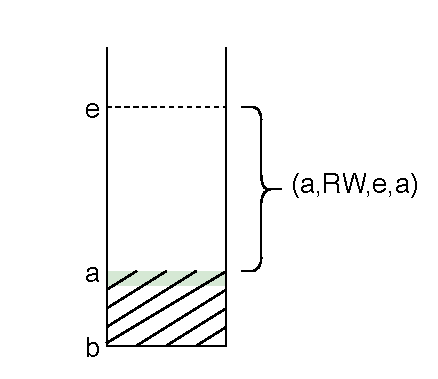
\includegraphics[scale=0.7]{images/wbcf_3.pdf}};
\end{tikzpicture}

\column{.5\textwidth} % Right column and width
\begin{center}
\begin{lstlisting}
push r_stk 1
scall r 
pop r_stk r_1
assert r_1 1
halt
\end{lstlisting}
\end{center}

\end{columns}

\begin{align*}
 		\mathcal{E}\interp{\Sigma}{pc} \triangleq&~\forall r, \mathcal{R}(\Sigma)(r) ~*~{\textsf{context}(\Sigma)(r[\textsf{\small PC}:=pc])}\\
 		&\sep~\textsc{WP}~\textsf{Seq (Instr Executable)}~\\
 		&\hspace{1cm}\{ v, v = HaltedV \implies \exists \Sigma ' r', \Sigma ' \sqsupseteq_{priv} \Sigma \\
 		&\hspace{1cm}* {\textsf{context}(\Sigma ')(r')}\}
 	\end{align*}

\end{frame}


\end{document} 